\documentclass[pdflatex,sn-mathphys-num]{sn-jnl}
\usepackage[T2A]{fontenc}
\usepackage{color}
\usepackage[utf8]{inputenc} % allow utf-8 input
\usepackage[T1]{fontenc}    % use 8-bit T1 fonts
\usepackage{hyperref}       % hyperlinks
\usepackage{url}            % simple URL typesetting
\usepackage{booktabs}       % professional-quality tables
\usepackage{amsfonts}       % blackboard math symbols
\usepackage{nicefrac}       % compact symbols for 1/2, etc.
\usepackage{microtype}      % microtypography
\usepackage{lipsum}
\usepackage{graphicx}
\usepackage{color}

\usepackage{tabularx}
\usepackage{amsthm,amsmath,amssymb}


\begin{document}
\begin{titlepage}
  \begin{center}
      \line(1,0){400}\\
      \huge{\bfseries{Eigen Value Caluclation}}
        \line(1,0){400}\\
  
 \textsc{\small Golla Shriram - AI24btech11010}
\end{center}  
\hspace{2cm}
\section{Introduction}
If $A$ is $n\times n$ matrix and $\mathbf{v}$ be a non-zero vector of length $n$. If it satisfies 
   \begin{align}
       A\mathbf{v} = \lambda \mathbf{v}
   \end{align}  
then $\lambda$ is known as \textbf{eigen value} which may be real or imaginary and $\mathbf{v}$ is \textbf{eigen vector}. Eigen values and Eigen vectors are very much useful in understanding the linear transformations and have many other applications in engineering and science. 
\\

      Eigen values are the roots for characteristic polynomial given by  $det(A-\lambda I) = 0$. The idea of directly finding the roots  is not viable as the computation difficulty largely increases with $n$ as stated by \textbf{Abel–Ruffini theorem} that it's impossible to solve all polynomial equations (of degree 5 or higher) using a general formula made up of basic operations and also there are unavoidable round-off error which cause sensitive changes to the roots of characteristic polynomial. Hence numerical methods are used to approximate the eigen value. 
      

\section{Algrothim Selection}
 Many iterative algorithms were devised to solve the eigenvalue problem by producing sequences that converge to the eigenvalues. 
 \begin{itemize}
\item QR algorithm
\item  Divide-and-conquer
\item  Laguerre iteration
\item  Jacobi eigenvalue algorithm
\item  Arnoldi and Lanczos algorithms
\end{itemize}

\subsection{QR - Algorithm}
 The QR algorithm uses \textbf{Schur decomposition} of a matrix. It is best applied on \textbf{dense matrices}.  The overall complexity is $\mathcal{O}(n^3)$ floating point operations. It has \textbf{cubic convergence rate}. It is not compatible for sparse matrices.

 \end{titlepage}
\subsection{Divide and Conquer}
 The divide and conquer algorithm as name suggest involves partitioning of eigenvalue problem into smaller eigenvalue problems, solving them and combining all the solutions to get desired solutions. The overall complexity is $\mathcal{O}(n^3)$ . It is best applied on Hermitian matrices. It has \textbf{ faster Cubic convergence}. It has high memory requirements .
 
\subsection{Laguerre iteration}
This algorithm is based on Laguerre method was designed for polynomials with real zeros and when these are distinct it gives strong convergence right from any starting value but it also applies well in complex plane. It is generally used to find a subset of eigenvalues instead of all eigen values with more degree pf accuracy.The overall complexity is $\mathcal{O}(n^2)$ for single eigenvalue and  $\mathcal{O}(n^3)$ for all eigenvalues. It has \textbf{cubic convergence}.


\subsection{Jacobi eigenvalue algorithm}
Jacobi eigenvalue algorithm is an iterative method to calculate the eigenvalues  of a real symmetric matrix by a sequence of Jacobi rotations. The  complexity is $\mathcal{O}(n^3)$. It has \textbf{quadratic convergence}. It can handle small matrices but when it comes for large matrices it is not viable. 
\subsection{ Arnoldi and Lanczos algorithms}
Arnoldi and Lanczos algorithms both are based on  Krylov subspace methods for finding eigen values. These methods are extremely good for finding eigen values of Large sparse matrices. Lanczos best works on \textbf{symmetric} mactries where Arnoldi works on \textbf{non symmetric} mactries . The complexities are $\mathcal{O}(mn^2)$ for Arnoldi and  $\mathcal{O}(mn)$for Lanczos for $m$ steps.
\begin{table}[h!]
\centering
\begin{tabular}{|l|l|l|l|}
\hline
\textbf{Algorithm} & \textbf{Matrix Type} & \textbf{Complexity} & \textbf{Convergence Rate} \\ \hline
QR Algorithm & Dense & $\mathcal{O}(n^3)$ &  Cubic (with shifts) \\ \hline
Divide and Conquer & Symmetric Tridiagonal &  $\mathcal{O}(n^3)$  & Faster Cubic \\ \hline

Laguerre Iteration & Polynomials/Subset & $\mathcal{O}(n^2)$   & Cubic (simple roots) \\ \hline
Jacobi Algorithm & Real Symmetric & $\mathcal{O}(n^3)$ & Quadratic \\ \hline
Arnoldi & General Sparse & $\mathcal{O}(mn^2)$ & Superlinear  \\ \hline
Lanczos & Symmetric Sparse & $\mathcal{O}(mn)$ & Superlinear  \\ \hline
\end{tabular}
\caption{Comparison of Eigenvalue Algorithms}
\label{tab:eigen_algorithms}
\end{table}


\newpage

\begin{figure}[h]
\centering 
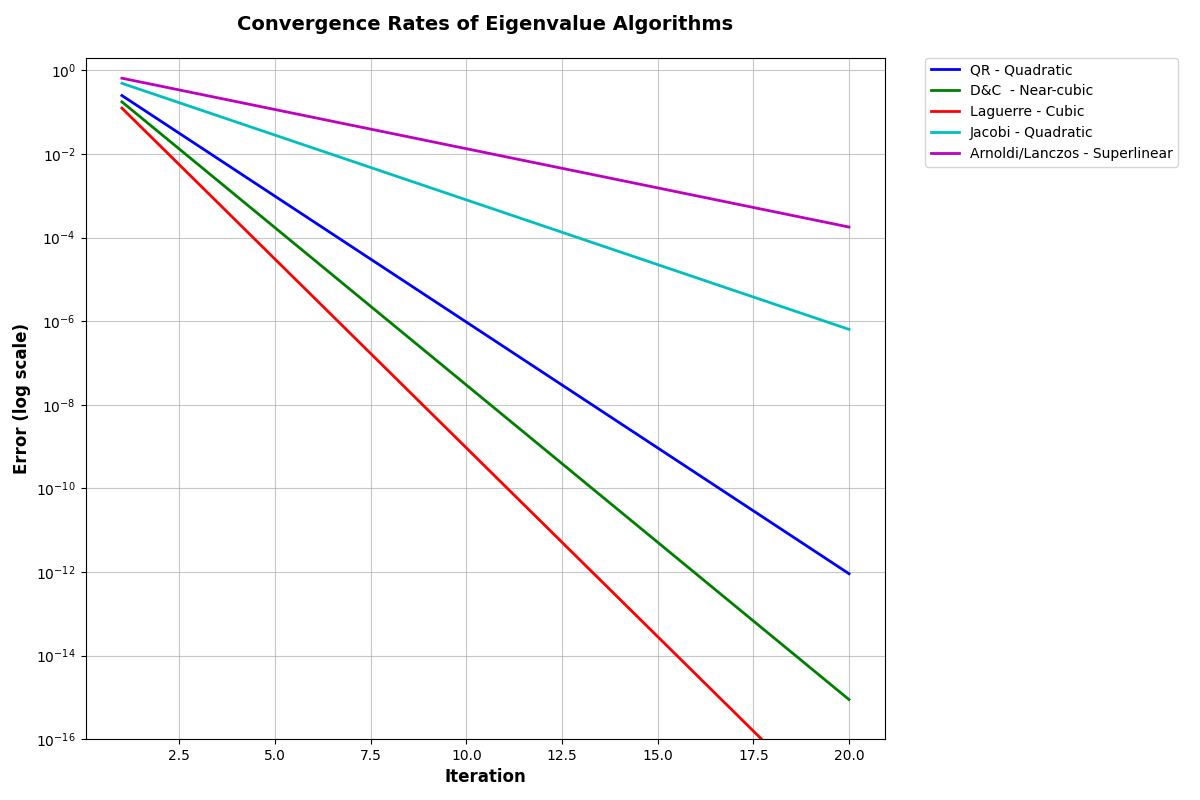
\includegraphics[width=15cm]{rate of convergence.png}
\end{figure}


On comparing above algorithms each algorithm has its own pros and cons but if i were to choose an eigen value solving algorithm i would choose QR algorithm because of its versatility with both symmetric and non - symmetric matrix , faster rate of convergence and its ability for handiling large set of matrices.

\section*{Algorithm Implementation}
\subsection*{QR- Algorithm}
The process involves of decomposition A into Q and R such that $A=QR$ , Q is an orthogonal matrix and R is upper triangular matrix. The idea is to start with a matrix $A$ and decompose it into $Q$ and $R$ then we construct another matrix $A_1$ such that $A_1 = RQ$. We then again decompose the matrix into $Q_1$ and $R_1$ such that $A_1=Q_1R_1$ where  $Q_1$ is an orthogonal matrix and $R_1$ is upper triangular matrix. We iterate k times until $A_k$ becomes converges closer to diagonal form, the diagonal elements of $A_k$ approximate the eigenvalues of the original matrix $A$.

    The QR decomposition can be done using  
     \begin{itemize}
\item Gram-Schmidt Process
\item  Householder Reflections
\item  Rotations
\item  Cholesky Decomposition
\end{itemize}


\subsection*{House holder Transformations }
 The most efficient and widely used is House holder Transformations it is preferred because of its stability and efficiency.

Start with A $n\times n $. We then extract the first column vector $x_1$ of A:
$$ x_1 = \begin{pmatrix} A_{11} \\A_{21}\\ \vdots \\ A_{n1} \end{pmatrix} \;     $$
We then caluclate norm of $x_1$ :
$$     ||x|| = \sqrt{ A^{2}_{11}+ A^{2}_{21}+\cdots+A^{2}_{n1}}$$
Next we define a householder vector $\mathbf{v_1}$  to create a reflection that eliminates the elements below the diagonal in the first column. This vector is given by 
$$  v_1  = x_1 - ||x||e_1$$
where $e_1 = \begin{pmatrix} 1 \\ 0 \\ \vdots\\0 \end{pmatrix} \; . $ We then find the unit vector in direction of $v_1$. Then House holder matrix $$H_1 = I  - 2 v_1v_1^{T} e_1  $$ 
Apply the Householder transformation matrix to obtain a new matrix $A_1 =H_1A$ we then apply Householder transformation to handle the submatrix of $A_1$ to generate $H_2$ until we find an $A_k$ is transformed into upper triangular matrix i.e $A_k = R $ and $Q = H_1H_2...H_k$ will result an orthogonal matrix such that
$$ A =QR$$
By using these values of $Q$ and $R$ we find values of $A_1$ and then consequently $A_k$ whose diagonal elements could be approximated as the eigen values of $A$

\newpage
\section{Testing of code}
In the following section we are going to compare the Basic Qr algorithm implementation with state of art - Numpy, linalg eigen value function. 
\iffalse
\begin{enumerate}
    \item $\begin{pmatrix}  
1 & 5 \\
6 & 9 
\end{pmatrix}$

eigen values by numpy  $\begin{bmatrix}
-1.78232998 \\ 11.78232998
\end{bmatrix}$

eigen values given by QR $\begin{bmatrix} -1.782330\\11.782330 \\\end{bmatrix}$

\item $\begin{pmatrix}  
6 & 4 & 1\\
7 & 12 & 9\\
23 & 87 & 1
\end{pmatrix}$

eigen values by Numpy $ \begin{bmatrix}
 36.68518825 \\  4.32581544 \\-22.0110037  
\end{bmatrix}$

eigen values given by QR $\begin{bmatrix} 36.685188\\-22.011004\\4.325815\end{bmatrix}$


\item $\begin{pmatrix}   \\
3 & 4 & 1& 6 & 9\\
2&0 & 6&2 & 3\\
5 & 7 & 1&7&8\\
12 &6 &5&5&1\\
41&8&7&1 &3\\

\end{pmatrix}$

eigen values by Numpy $ \begin{bmatrix}
  29.84163693 \\ -18.76990641  \\ 4.93433348 \\   0.89484631 \\ -4.90091031
  
\end{bmatrix}$

eigen values given by QR $\begin{bmatrix} 29.841637 \\
-18.769906 \\
4.934333\\
-4.900910\\
0.894846\end{bmatrix}$



\item  \begin{pmatrix}
34 & 92 & 56 & 74 & 61 & 15 & 88 & 47 & 13 & 29 \\
26 & 74 & 58 & 91 & 49 & 36 & 59 & 11 & 82 & 43 \\
53 & 71 & 34 & 60 & 80 & 2 & 17 & 68 & 99 & 21 \\
14 & 27 & 63 & 41 & 55 & 9 & 85 & 95 & 30 & 70 \\
76 & 38 & 52 & 73 & 23 & 78 & 66 & 83 & 65 & 10 \\
69 & 77 & 28 & 94 & 42 & 50 & 7 & 31 & 12 & 75 \\
8 & 33 & 57 & 20 & 40 & 86 & 97 & 60 & 64 & 4 \\
24 & 64 & 1 & 81 & 90 & 46 & 48 & 13 & 93 & 53 \\
79 & 98 & 85 & 17 & 16 & 18 & 72 & 25 & 22 & 67 \\
37 & 5 & 84 & 62 & 39 & 51 & 19 & 3 & 50 & 28
\end{pmatrix}

eigen values by Numpy $ \begin{bmatrix}
496.1665913  +0.j    \\     -82.44133521+23.88452113j\\
 -82.44133521-23.88452113j\\ -24.98345636+60.29862066j\\
 -24.98345636-60.29862066j \\  1.59109661+69.58203827j\\
   1.59109661-69.58203827j \\ 33.15250429+48.03333842j\\
  33.15250429-48.03333842j \\ 65.19579005 +0.j        
\end{bmatrix}$

eigen values given by QR $\begin{bmatrix} 
496.166591\\
-82.441335 + 23.884521i \\
-82.441335 - 23.884521i\\
1.591097 + 69.582038i\\
1.591097 - 69.582038i\\
-24.859804 + 60.877278i\\
-24.859804 - 60.877278i\\
64.948485\\
33.152504 + 48.033338i\\
33.152504 - 48.033338i\\
\end{bmatrix}$
\end{enumerate}

\fi


\begin{table}[h!]
\resizebox{12cm}{!} {
\begin{tabular}{|c|c|c|}
\hline
\textbf{Matrix} & \textbf{Eigenvalues by Numpy} & \textbf{Eigenvalues by QR} \\
\hline
$\begin{pmatrix}  
1 & 5 \\ 
6 & 9 
\end{pmatrix}$ & 
\begin{tabular}{c} \\
-1.78232998 \\ 
11.78232998 \\
\\ \end{tabular} & 
\begin{tabular}{c} 
-1.782330 \\ 
11.782330 
\end{tabular} \\
\hline
$\begin{pmatrix}  
6 & 4 & 1 \\ 
7 & 12 & 9 \\ 
23 & 87 & 1 
\end{pmatrix}$ & 
\begin{tabular}{c} \\
36.68518825 \\ 
4.32581544 \\ 
-22.0110037 \\
\\\end{tabular} & 
\begin{tabular}{c} 
36.685188 \\ 
-22.011004 \\ 
4.325815 
\end{tabular} \\
\hline
$\begin{pmatrix}  
3 & 4 & 1 & 6 & 9 \\ 
2 & 0 & 6 & 2 & 3 \\ 
5 & 7 & 1 & 7 & 8 \\ 
12 & 6 & 5 & 5 & 1 \\ 
41 & 8 & 7 & 1 & 3 
\end{pmatrix}$ & 
\begin{tabular}{c} \\
29.84163693 \\ 
-18.76990641 \\ 
4.93433348 \\ 
0.89484631 \\ 
-4.90091031 \\
\\ \end{tabular} & 
\begin{tabular}{c} 
29.841637 \\ 
-18.769906 \\ 
4.934333 \\ 
-4.900910 \\ 
0.894846 
\end{tabular} \\
\hline
$\begin{pmatrix} 
34 & 92 & 56 & 74 & 61 & 15 & 88 & 47 & 13 & 29 \\ 
26 & 74 & 58 & 91 & 49 & 36 & 59 & 11 & 82 & 43 \\ 
53 & 71 & 34 & 60 & 80 & 2 & 17 & 68 & 99 & 21 \\ 
14 & 27 & 63 & 41 & 55 & 9 & 85 & 95 & 30 & 70 \\ 
76 & 38 & 52 & 73 & 23 & 78 & 66 & 83 & 65 & 10 \\ 
69 & 77 & 28 & 94 & 42 & 50 & 7 & 31 & 12 & 75 \\ 
8 & 33 & 57 & 20 & 40 & 86 & 97 & 60 & 64 & 4 \\ 
24 & 64 & 1 & 81 & 90 & 46 & 48 & 13 & 93 & 53 \\ 
79 & 98 & 85 & 17 & 16 & 18 & 72 & 25 & 22 & 67 \\ 
37 & 5 & 84 & 62 & 39 & 51 & 19 & 3 & 50 & 28 
\end{pmatrix}$ & 
\begin{tabular}{c} \\
496.1665913 \\ 
-82.44133521 + 23.88452113i \\ 
-82.44133521 - 23.88452113i \\ 
-24.98345636 + 60.29862066i \\ 
-24.98345636 - 60.29862066i \\ 
1.59109661 + 69.58203827i \\ 
1.59109661 - 69.58203827i \\ 
33.15250429 + 48.03333842i \\ 
33.15250429 - 48.03333842i \\ 
65.19579005 \\
\\ \end{tabular} & 
\begin{tabular}{c} 
496.166591 \\ 
-82.441335 + 23.884521i \\ 
-82.441335 - 23.884521i \\ 
1.591097 + 69.582038i \\ 
1.591097 - 69.582038i \\ 
-24.859804 + 60.877278i \\ 
-24.859804 - 60.877278i \\ 
64.948485 \\ 
33.152504 + 48.033338i \\ 
33.152504 - 48.033338i 
\end{tabular} \\
\hline
\end{tabular} }

\label{tab:eigenvalues_comparison}
\end{table}

The code can handle really well upto certain limit when we take large values the efficiency of code is reduced and takes time, we also need to increase number of iterations and to get better values reduce tolerance.


\end{document} 
